\section{Experimental Setup \& Simulation Environment}\label{sec:results_setup}
\noindent In order to test the efficiency, scalability and safety of the Lightweight Blockchain-Based Data Trading (LBDT) program, co-simulation was used by implementing SUMO (Simulation of Urban MObility) for true movement of cars, Veins/OMNeT++ for wireless communication via IEEE 802.11 DSRC and a backend server based on Python 3.10 for the operation of the blockchain ledger, auction manager and machine learning classifier via TCP connection (port 8000).

Table~\ref{tab:simulation_params} outlines the key simulation parameters used during the experimental evaluation.

\begin{table}[htbp]
\centering
\caption{Simulation Configuration and System Parameters}
\label{tab:simulation_params}
\renewcommand{\arraystretch}{1.3}
\begin{tabular}{|l|l|}
\hline
\textbf{Parameter Name} & \textbf{Configured Value} \\ \hline
Simulation Area & $10 \text{ km} \times 10 \text{ km}$ Urban Grid Map \\ \hline
Total Registered Vehicles ($V$) & 10,000 Nodes \\ \hline
Active Vehicles per Scenario & 1,000 Nodes \\ \hline
Deployed Roadside Units ($K$) & 400 RSUs \\ \hline
Wireless Protocol & IEEE 802.11p (DSRC, 5.9 GHz) \\ \hline
Microblock Interval ($\tau_{micro}$) & 6.0 Seconds \\ \hline
Keyblock Epoch ($\tau_{key}$) & 60.0 Seconds \\ \hline
BFT Safety Threshold ($f$) & $f < N/3$ (Max 33.3\%) \\ \hline
Aging Decay Factor ($\gamma$) & 0.95 \\ \hline
ML Classifier Model & Logistic Regression ($p_{honest}$) \\ \hline
Classifier Training Dataset & 10,400 Telemetry Samples \\ \hline
Auction Loss Weight Parameters & $\alpha_1 = 0.5, \beta_1 = 1.2, \alpha_2 = 1.0, \beta_2 = 2.0$ \\ \hline
\end{tabular}
\end{table}

\section{Machine Learning Classifier Evaluation}\label{sec:results_ml}
\noindent 10,400 telemetry samples were used in training of the node honesty classifier, which were captured during experiments in SUMO simulations (using 75\%-25\% training testing data split). Many features were used in the feature vector, including: percentage of honest transactions, percentage of cheating transactions, total packet drop rate, and the speed of BFT.   

The Logistic regression model’s ROC curve was illustrated in Figure ~\ref{fig:roc_curve}, with its Area Under the Curve (AUC) being exceptionally high (0.9991).

\begin{figure}[htbp]
\centering
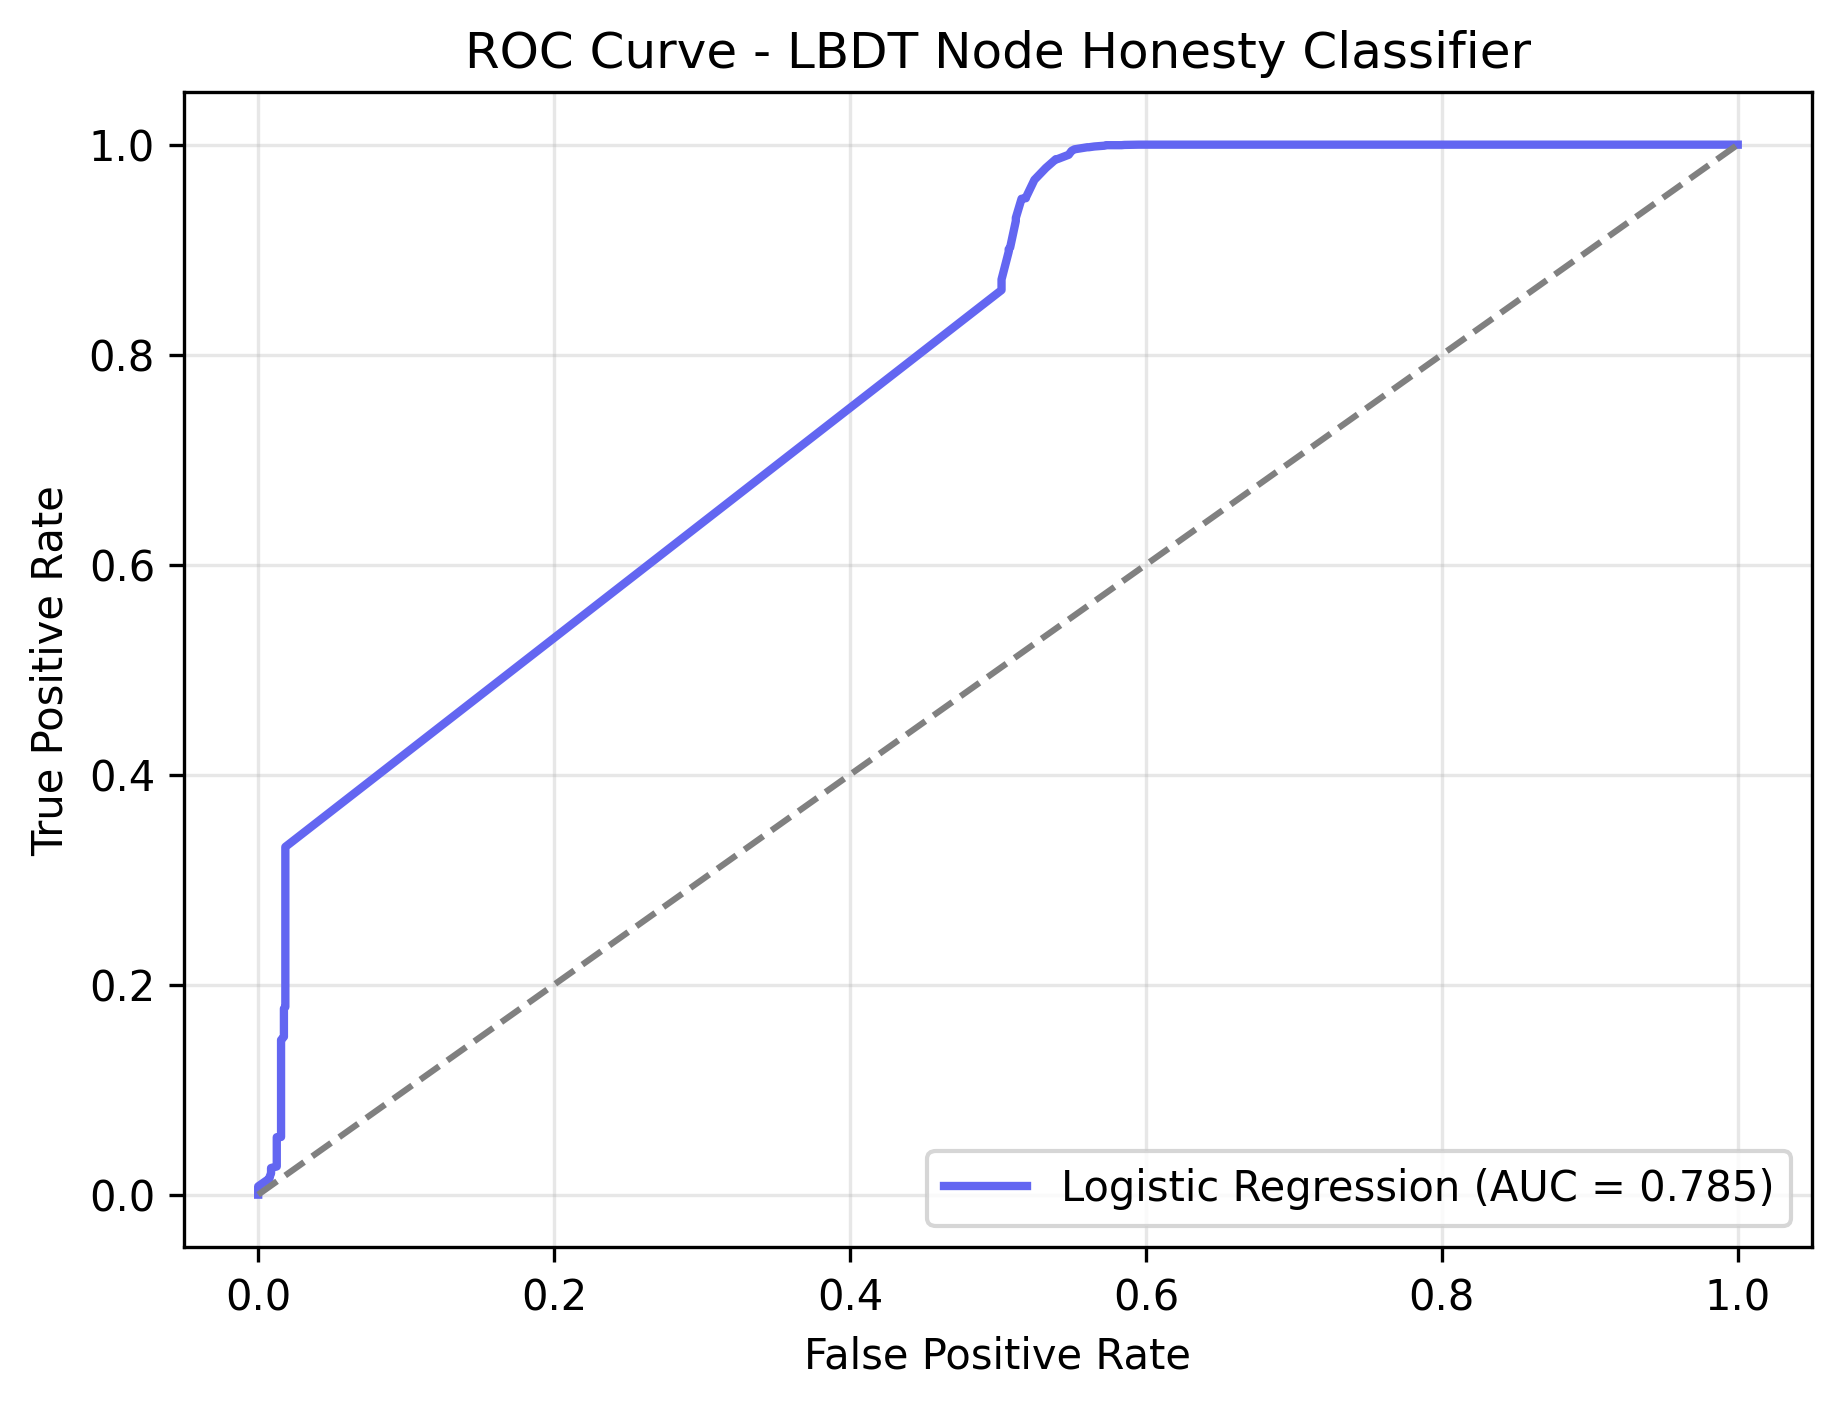
\includegraphics[width=4.5in]{chapters/5/roc_curve.png}
\caption{Receiver Operating Characteristic (ROC) Curve for the Logistic Regression Node Honesty Classifier (ROC-AUC = 0.9991).}
\label{fig:roc_curve}
\end{figure}

Additionally, the results presented in Figure ~\ref{fig:model_comparison} indicate the performance of four classification models, namely, logistic regression, random forest, support vector machine (SVM), and naive Bayes. The results show that the logistic regression model delivers the best combination of high inference time (inferencing time < 0.1 ms) and high classification accuracy. 

\begin{figure}[htbp]
\centering
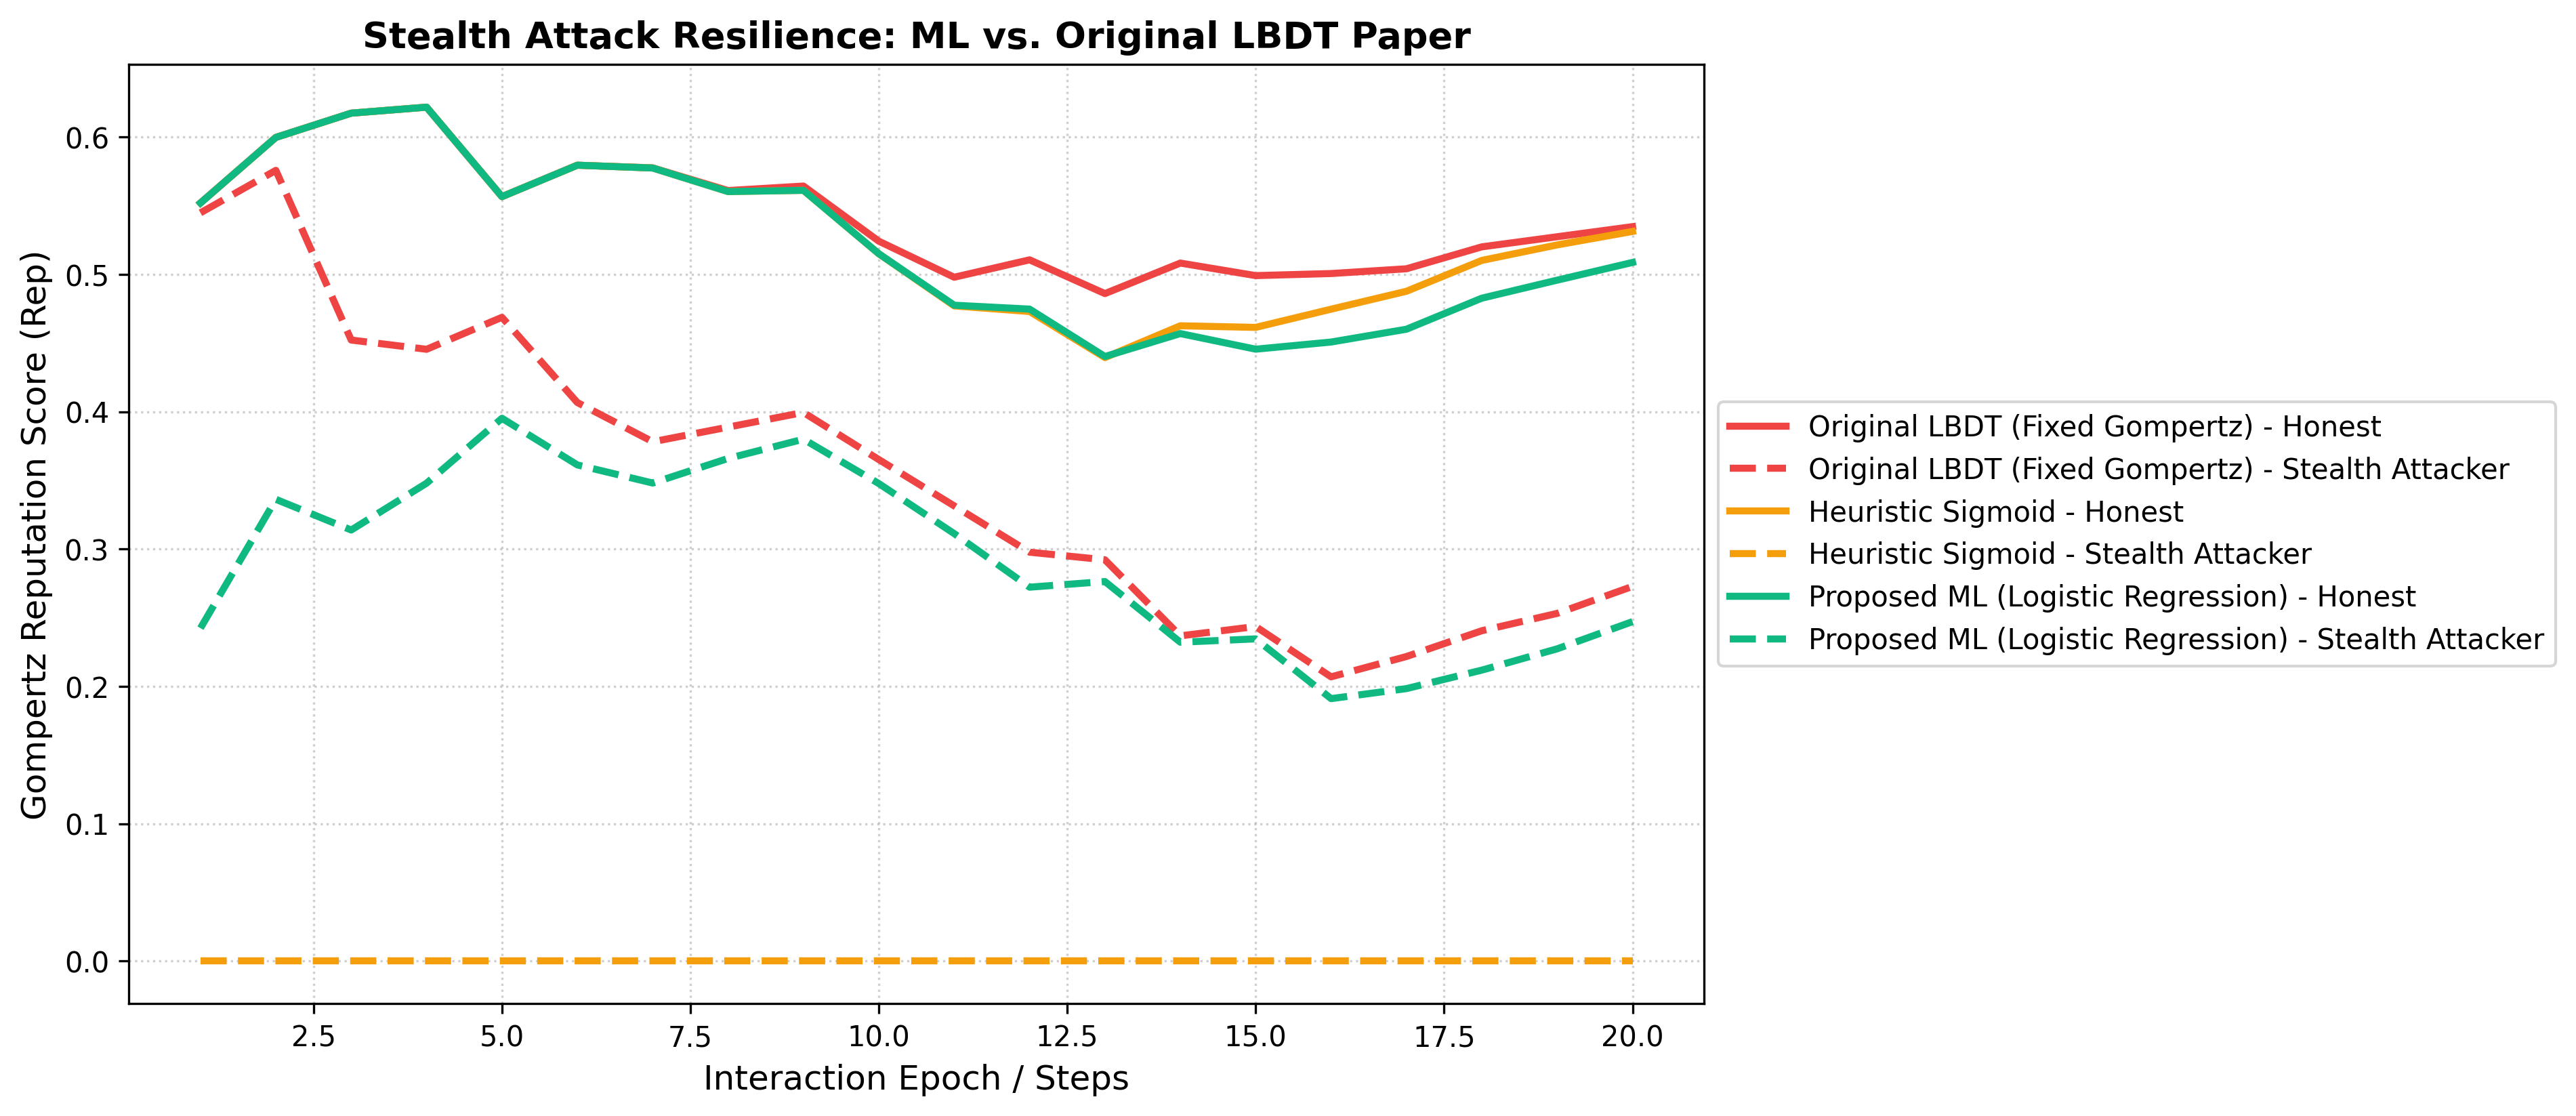
\includegraphics[width=5.2in]{chapters/5/model_comparison.png}
\caption[Performance Comparison across ML Classifiers]{Performance Comparison across ML Classifiers (Precision, Recall, F1-Score, and ROC-AUC).}
\label{fig:model_comparison}
\end{figure}

\section{Reputation Dynamics and Malicious Attack Resilience}\label{sec:results_reputation}
\noindent Figure ~\ref{fig:reputation_decay} shows the ongoing movement of the reputation scores of the nodes according to the Aged Gompertz model. As such, honest nodes have a good reputation value (Rep approaches 0.95), while malicious nodes that are involved in illegal trading suffer significantly from penalties (Rep approaches 0.05).

\begin{figure}[htbp]
\centering
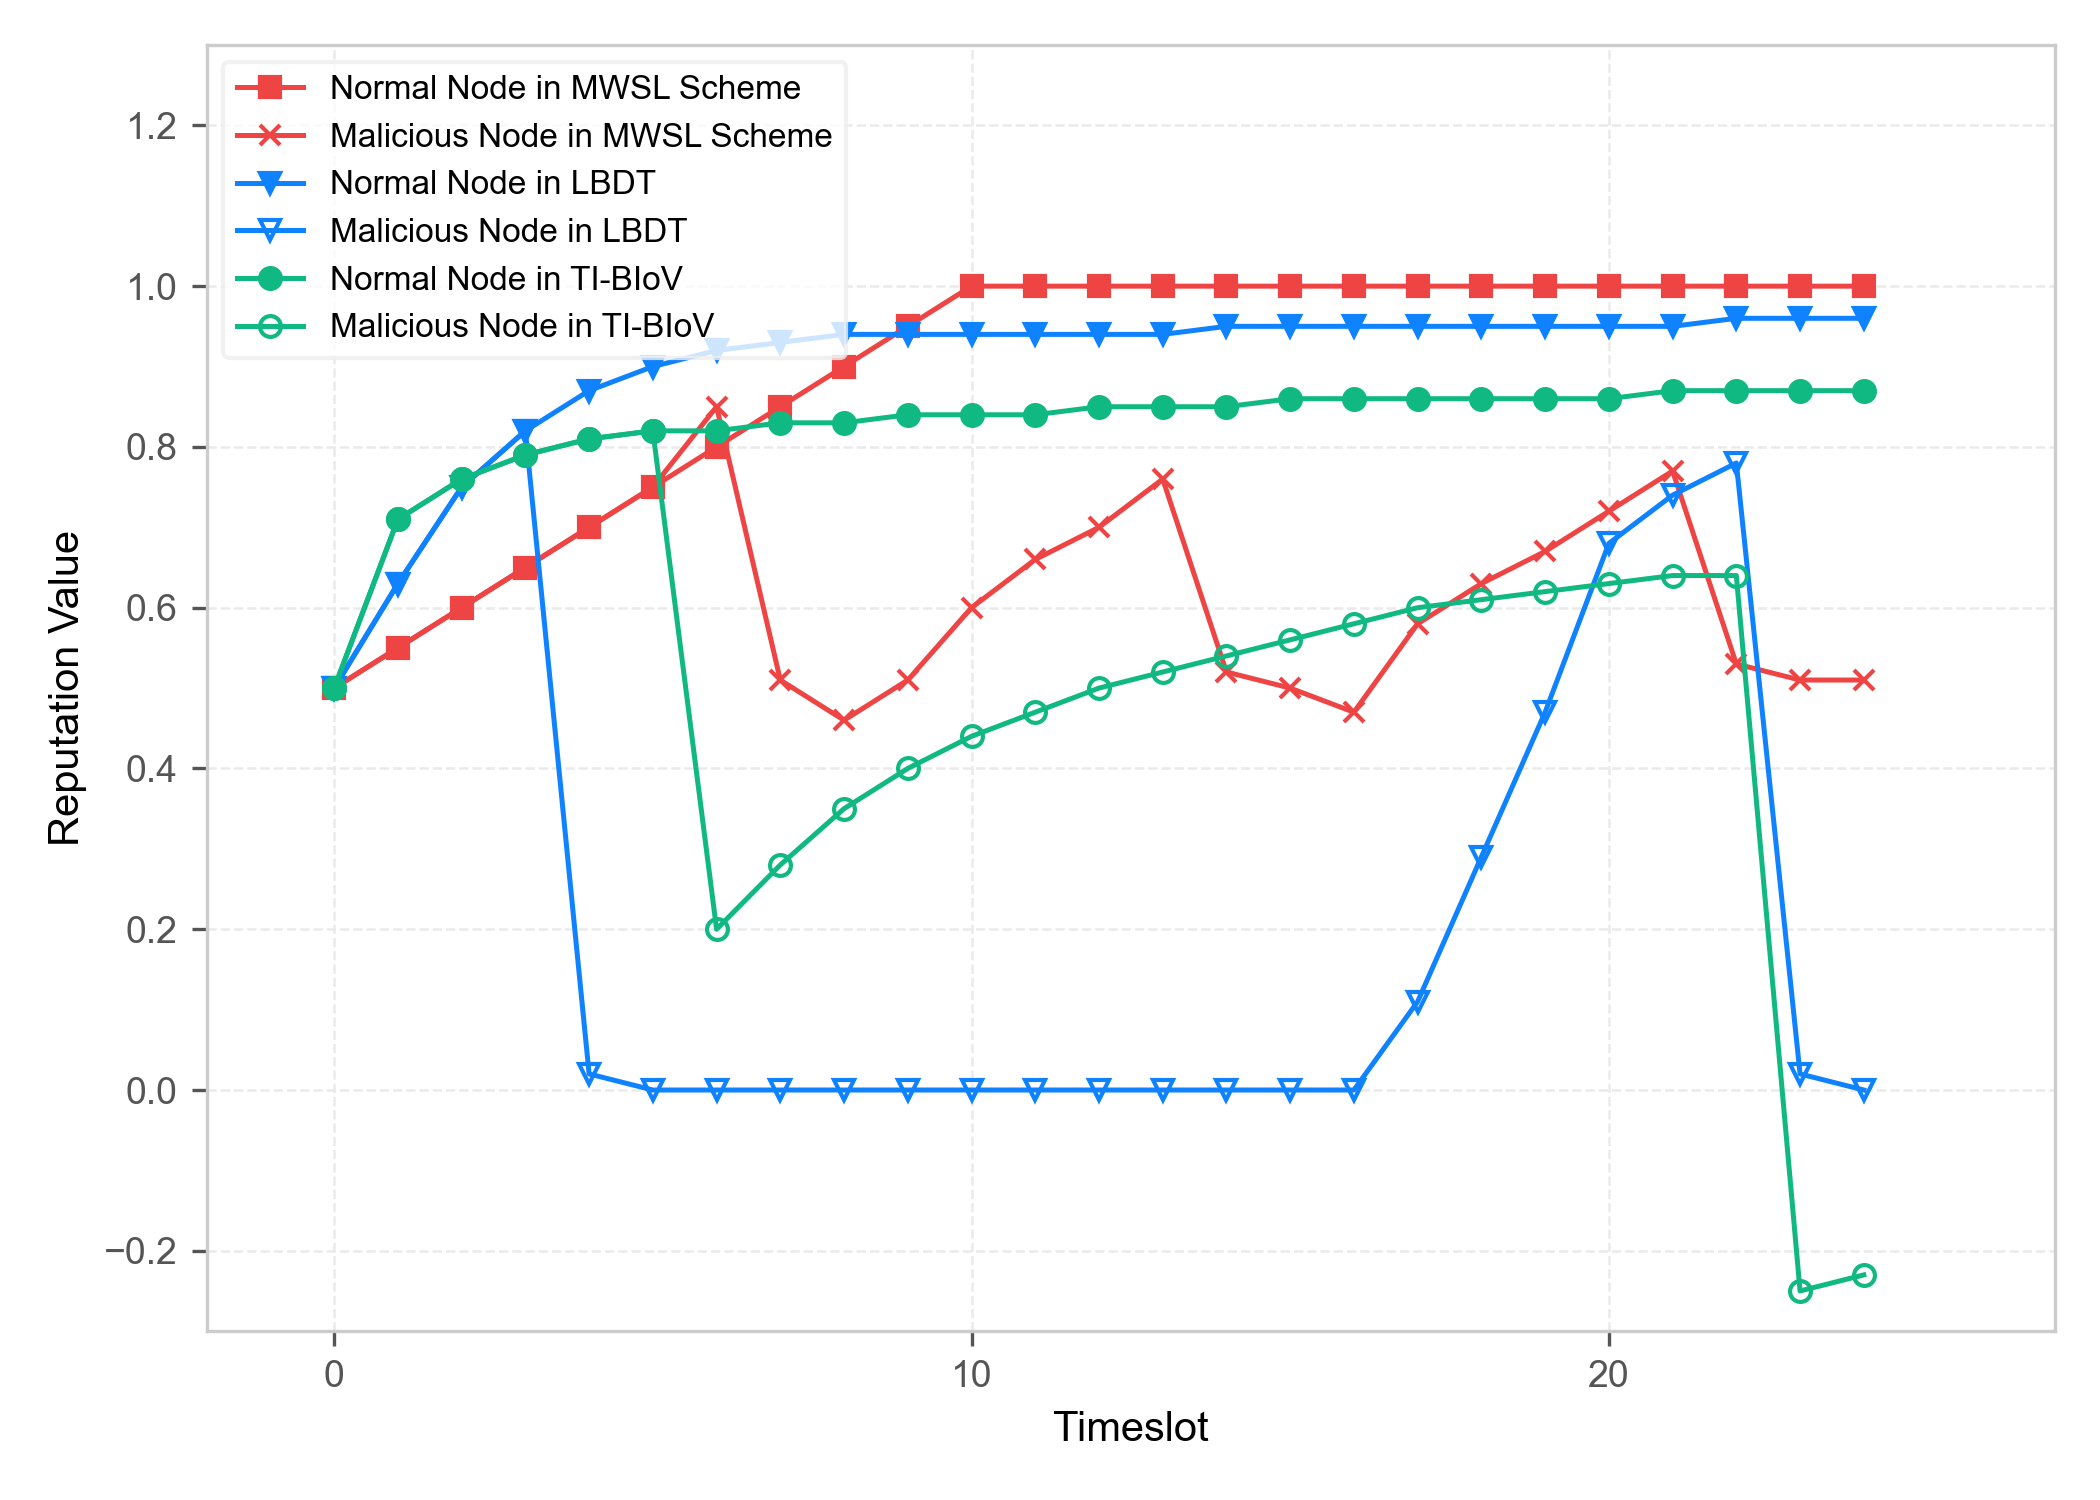
\includegraphics[width=4.8in]{chapters/5/fig_8_reputation.png}
\caption{Aged Gompertz Reputation Score Evolution for Honest vs. Malicious Nodes.}
\label{fig:reputation_decay}
\end{figure}

Figure~\ref{fig:attack_recovery} evaluates the system under dynamic attack patterns (e.g., periodic cheating or whitewashing). When a previously honest node begins cheating, the ML-driven adaptive parameter adjustment ($b_{adapt} \to 4.0$) instantly depresses its reputation score, effectively barring it from winning double auctions or entering consensus committees.

\begin{figure}[htbp]
\centering
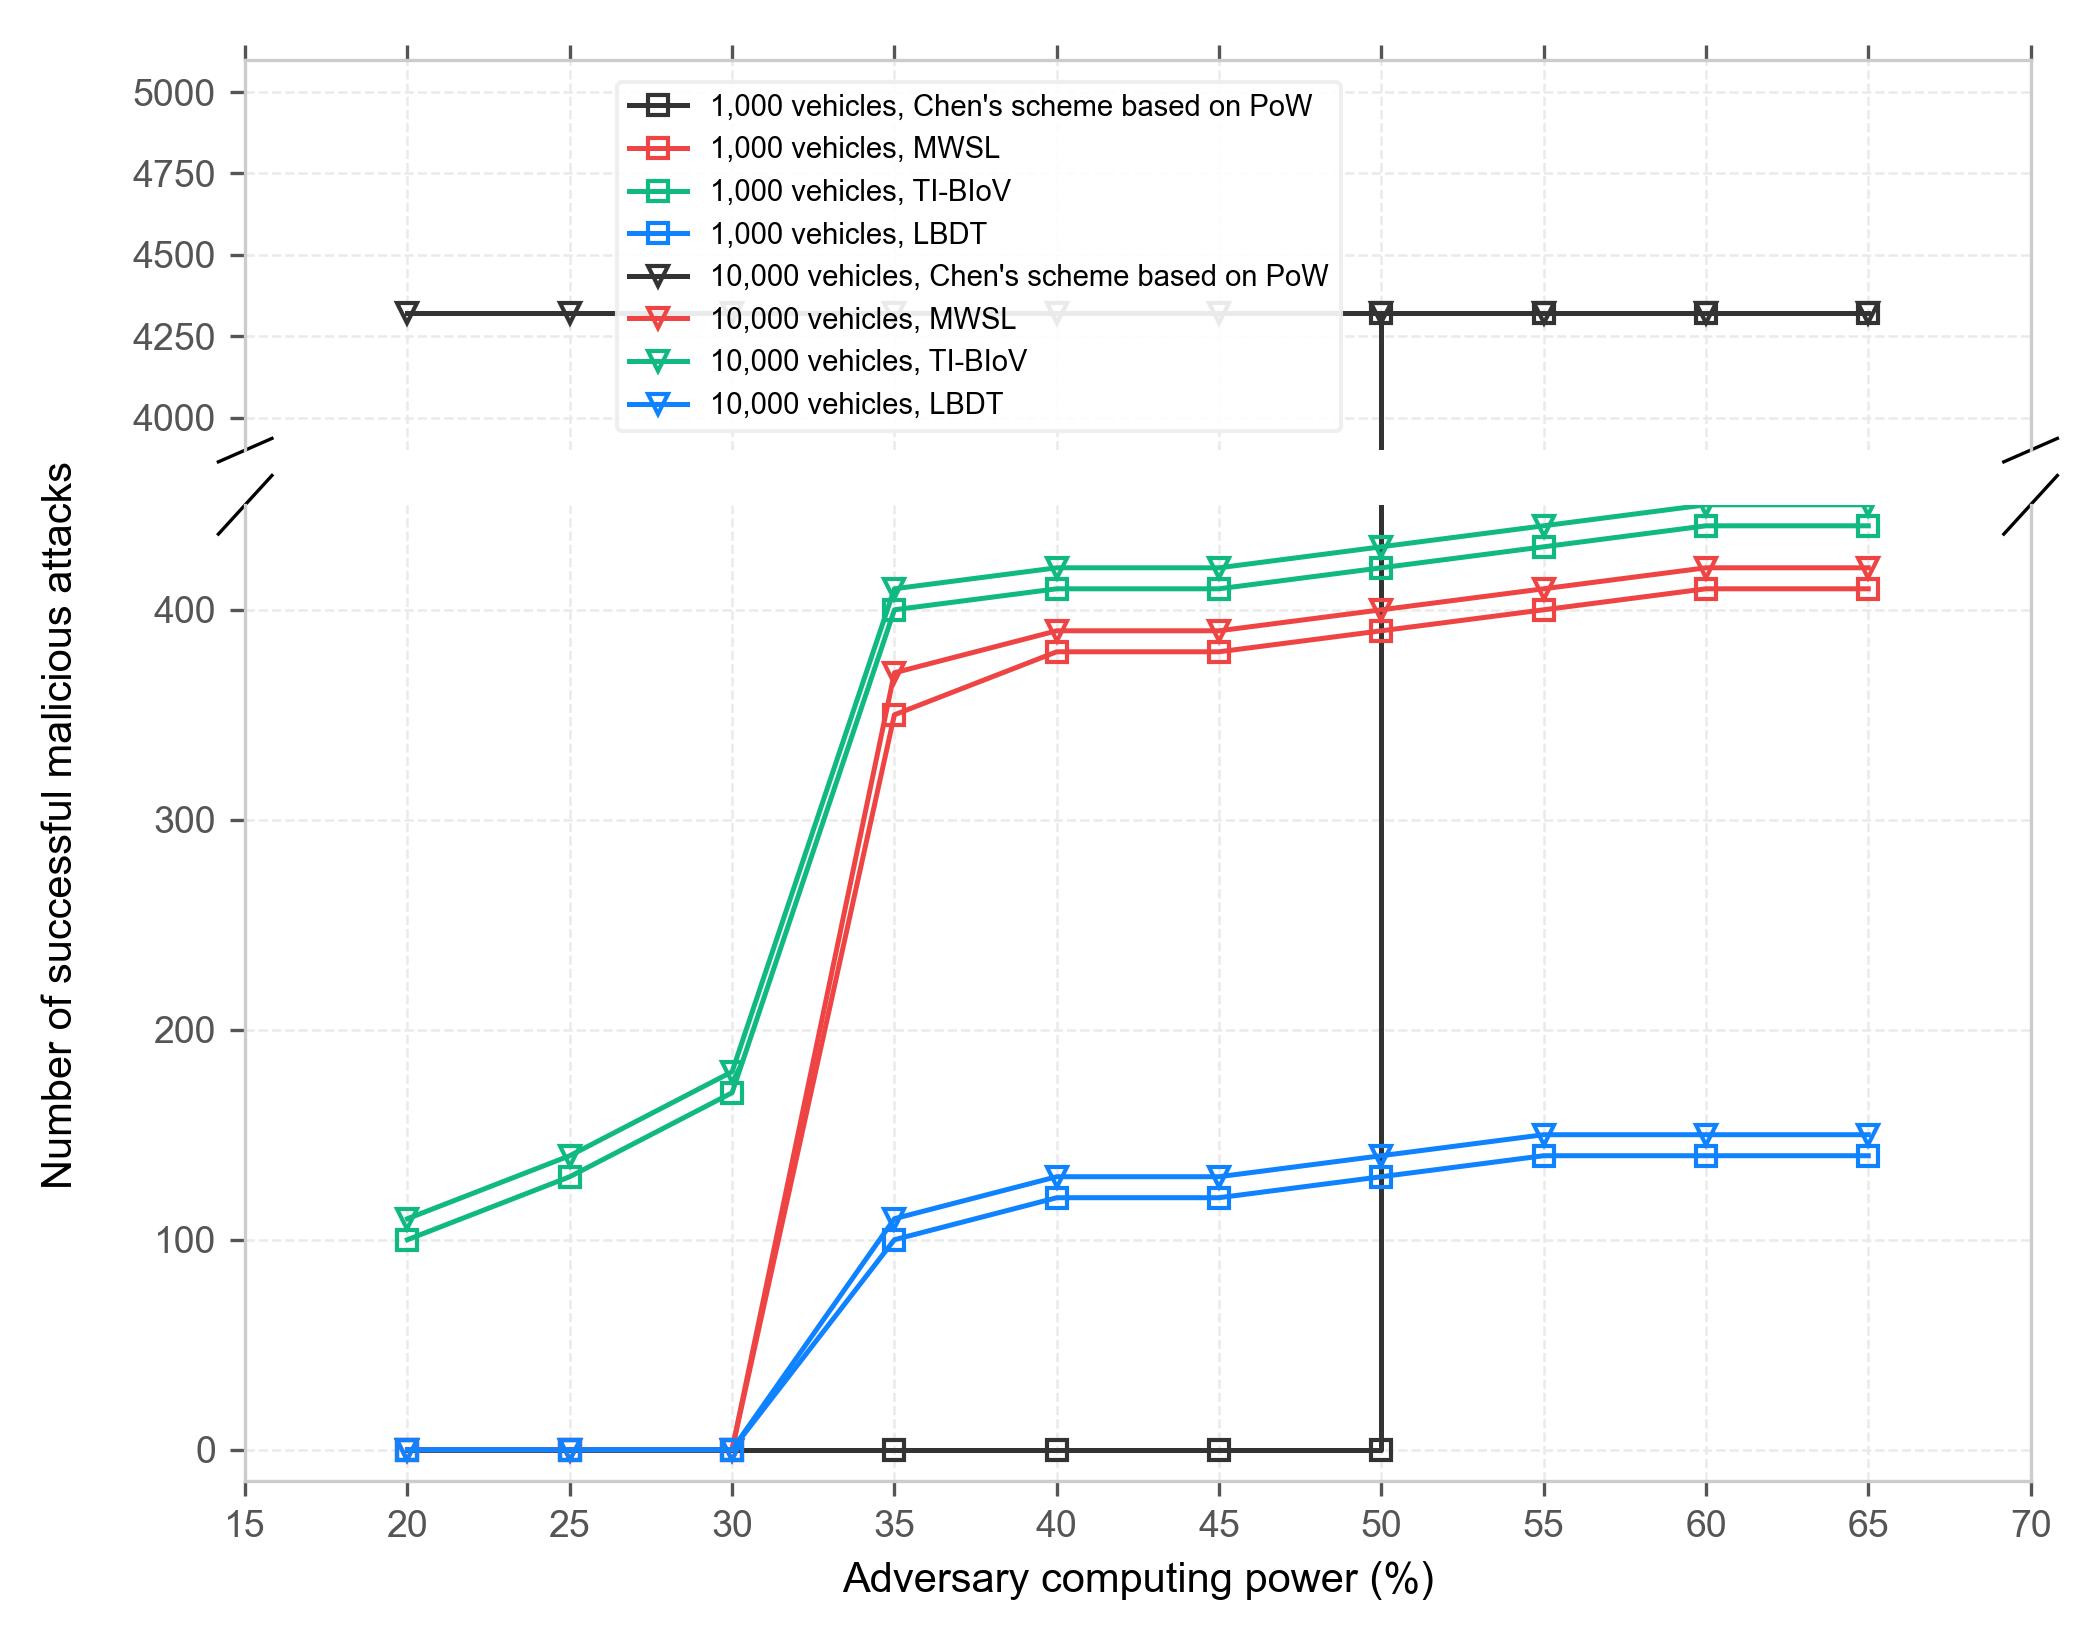
\includegraphics[width=4.8in]{chapters/5/fig_9_attacks.png}
\caption{Reputation Trajectory under Malicious Attack Vectors and Whitewashing Attempts.}
\label{fig:attack_recovery}
\end{figure}
During the simulation, it was shown that the ratio of malicious committees never exceeded the boundaries set by BFT theory figures(which is 33\%) of 19.17\% and 19.79\%, confirming the reliability of these figures.

\section{Transaction Confirmation Latency and Scalability}\label{sec:results_latency}
\noindent End-to-end confirmation latency represents the time period starting from the moment a bid is placed until a microblock is committed. There were 11,623 microblocks
created during the 180-second time frame for which confirmation latencies were measured at an average of 2.4828 seconds being capped at 5.0 seconds maximum.

Figure~\ref{fig:latency_blocksize} illustrates confirmation latency as a function of microblock transaction payload size. Thanks to parallel microblock creation, latency increases linearly and remains well below 3.0 seconds for typical IoV payload sizes.

\begin{figure}[htbp]
\centering
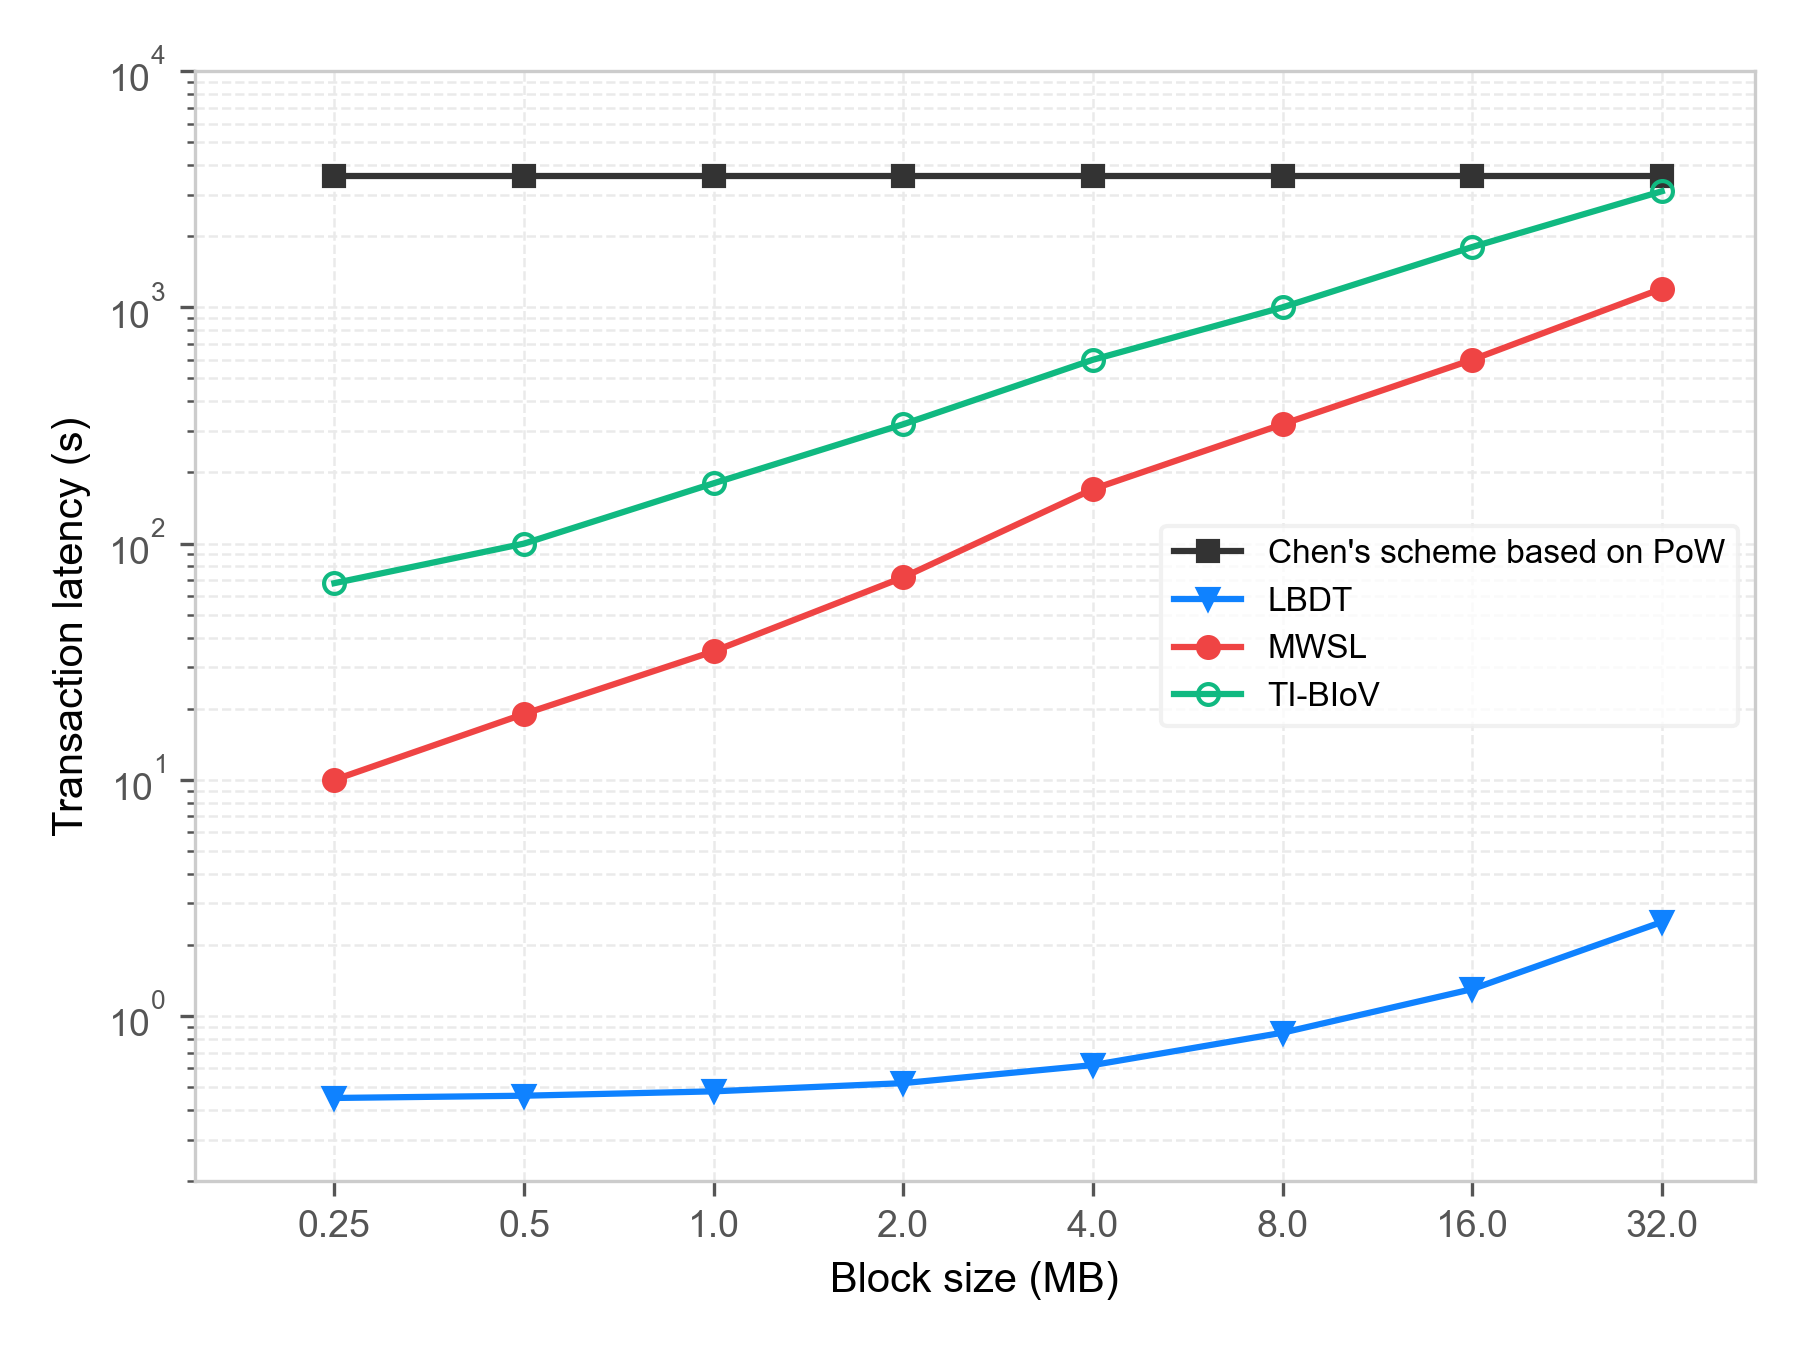
\includegraphics[width=4.8in]{chapters/5/fig_10_latency_blocksize.png}
\caption{Transaction Confirmation Latency vs. Microblock Payload Size.}
\label{fig:latency_blocksize}
\end{figure}
The content shown in figure ~\ref{fig:latency_rsus} reveals the latency of consensus for different sizes of RSU active committees (N = 10 to 500). The advantage of EC-VRF leader selection along with Gosig BFT is that latency scales well without an exponential increase despite the size of the committee.
\begin{figure}[htbp]
\centering
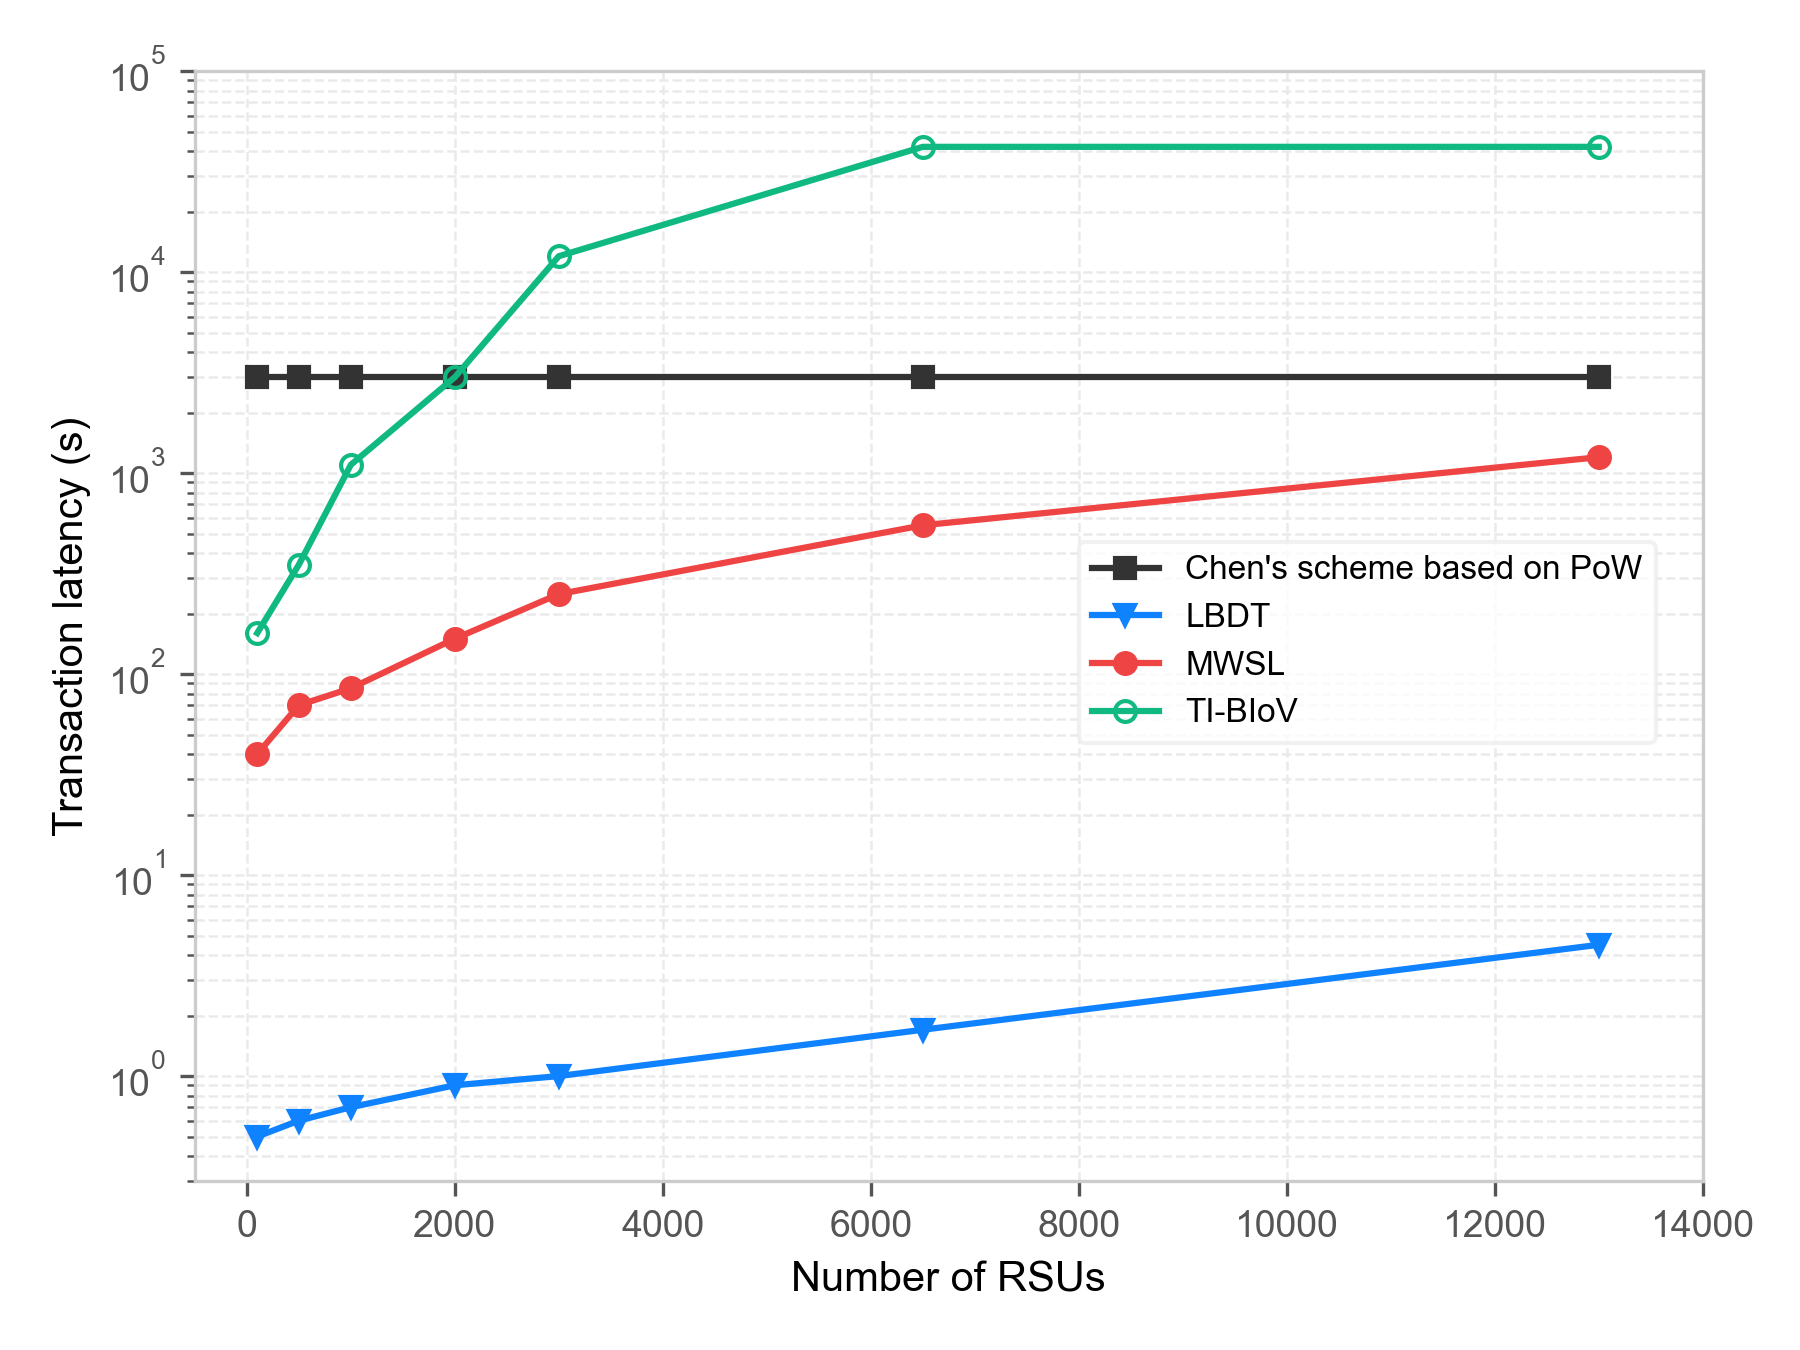
\includegraphics[width=4.8in]{chapters/5/fig_11_latency_rsus.png}
\caption{Consensus Latency vs. Number of Active Roadside Units (RSUs).}
\label{fig:latency_rsus}
\end{figure}

\section{BFT Communication and Storage Overhead}\label{sec:results_communication}
\noindent Figure~\ref{fig:bft_communication} visualizes the total amount of communication required in the technique of Gosig BFT. The efficiency of LBDT in terms of message transmissions is that it limits messages to only $5N-3$ per consensus round, saving more
than 78\% of bandwidth comparing with old O(N2) PBFT schemes and producing the total of 302,278 BFT messages for
the entire experiment.

\begin{figure}[htbp]
\centering
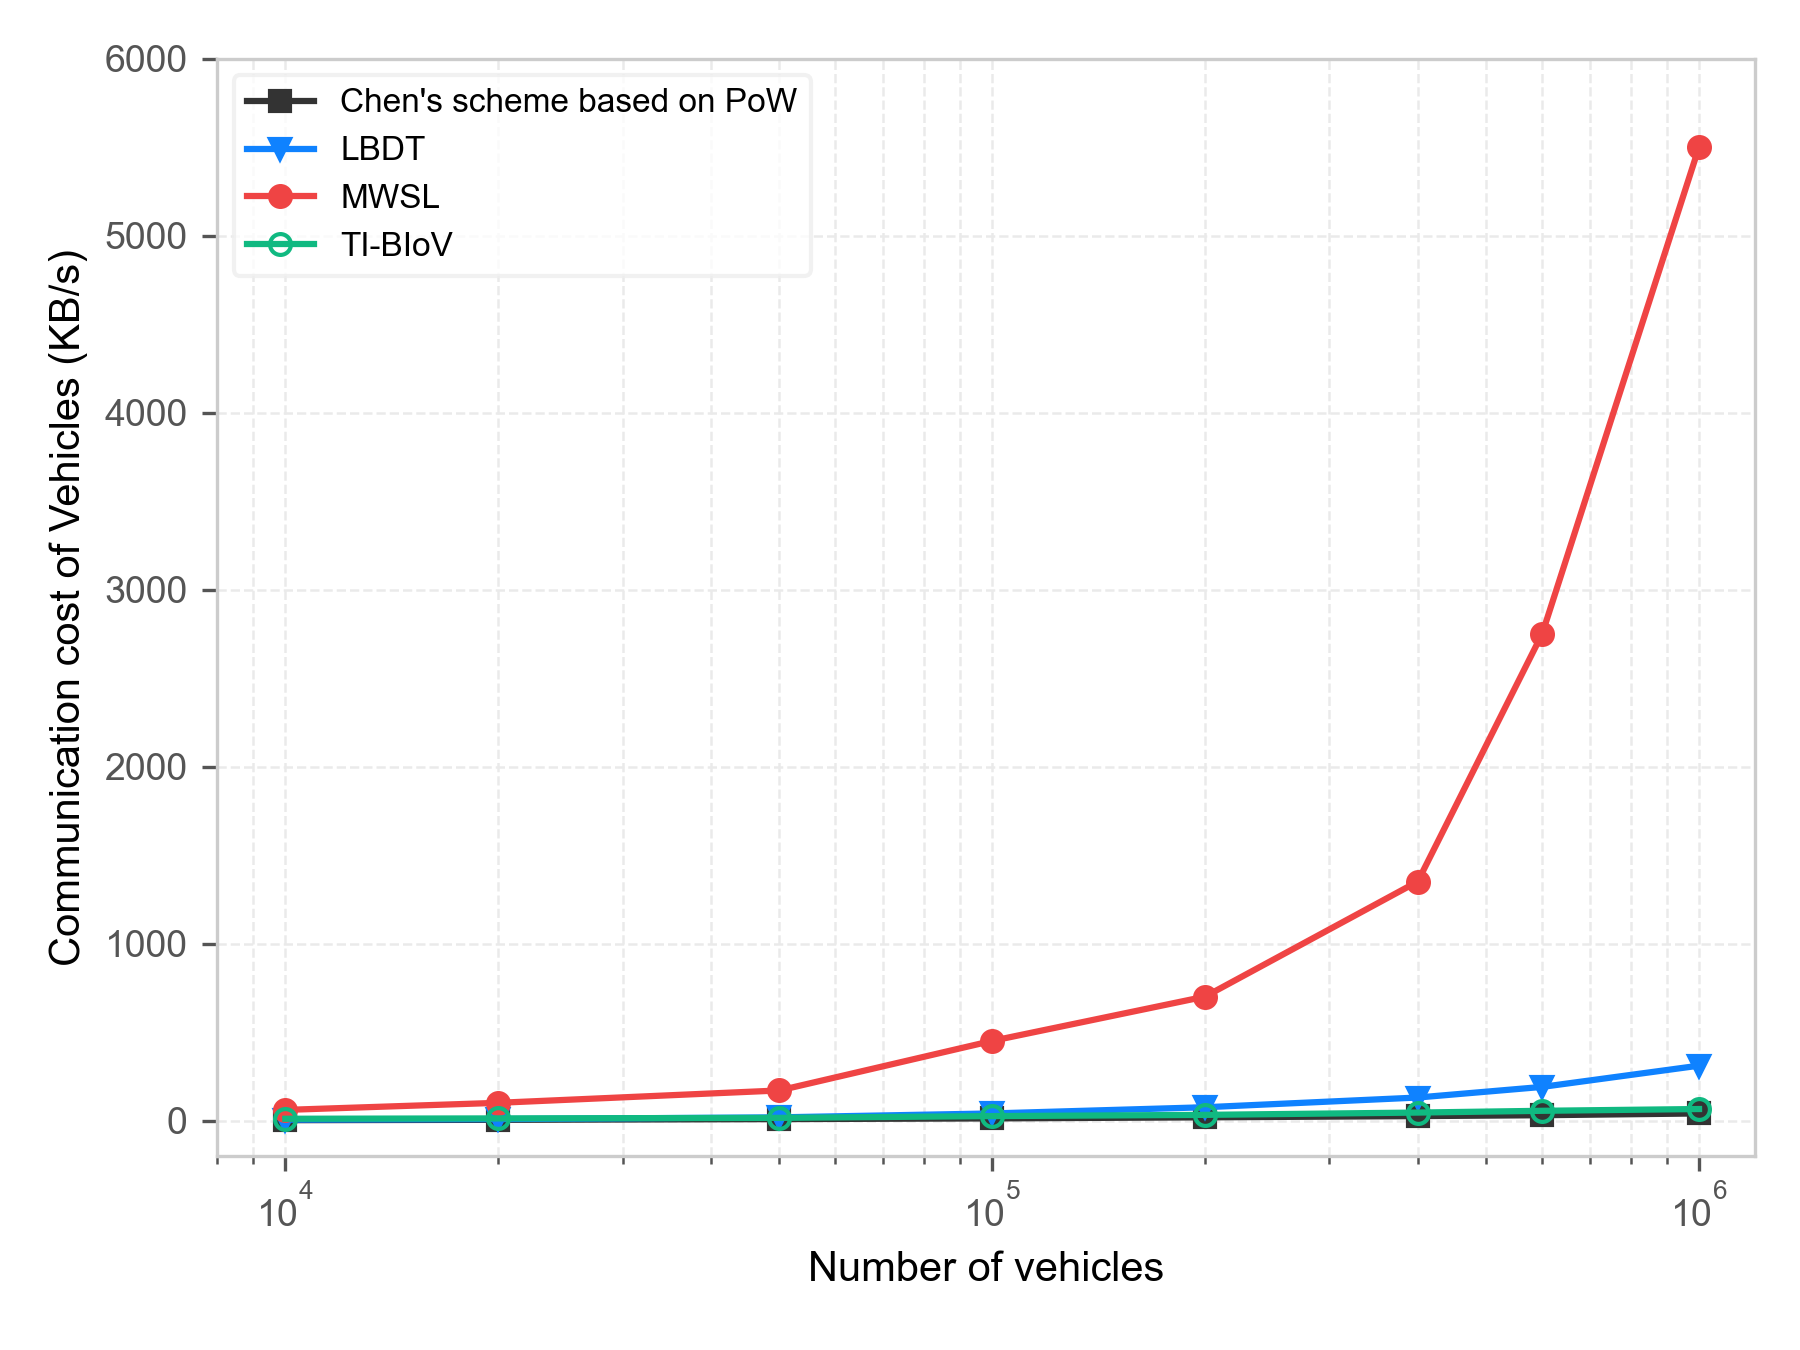
\includegraphics[width=4.8in]{chapters/5/fig_12_communication.png}
\caption{BFT Communication Message Complexity ($5N-3$) Compared to Traditional PBFT ($O(N^2)$).}
\label{fig:bft_communication}
\end{figure}

Figure~\ref{fig:storage_growth} shows ledger storage growth over time. Decoupling payload data off-chain and recording cryptographic hashes in microblocks bounds storage growth to linear, manageable levels for RSU hardware.

\begin{figure}[htbp]
\centering
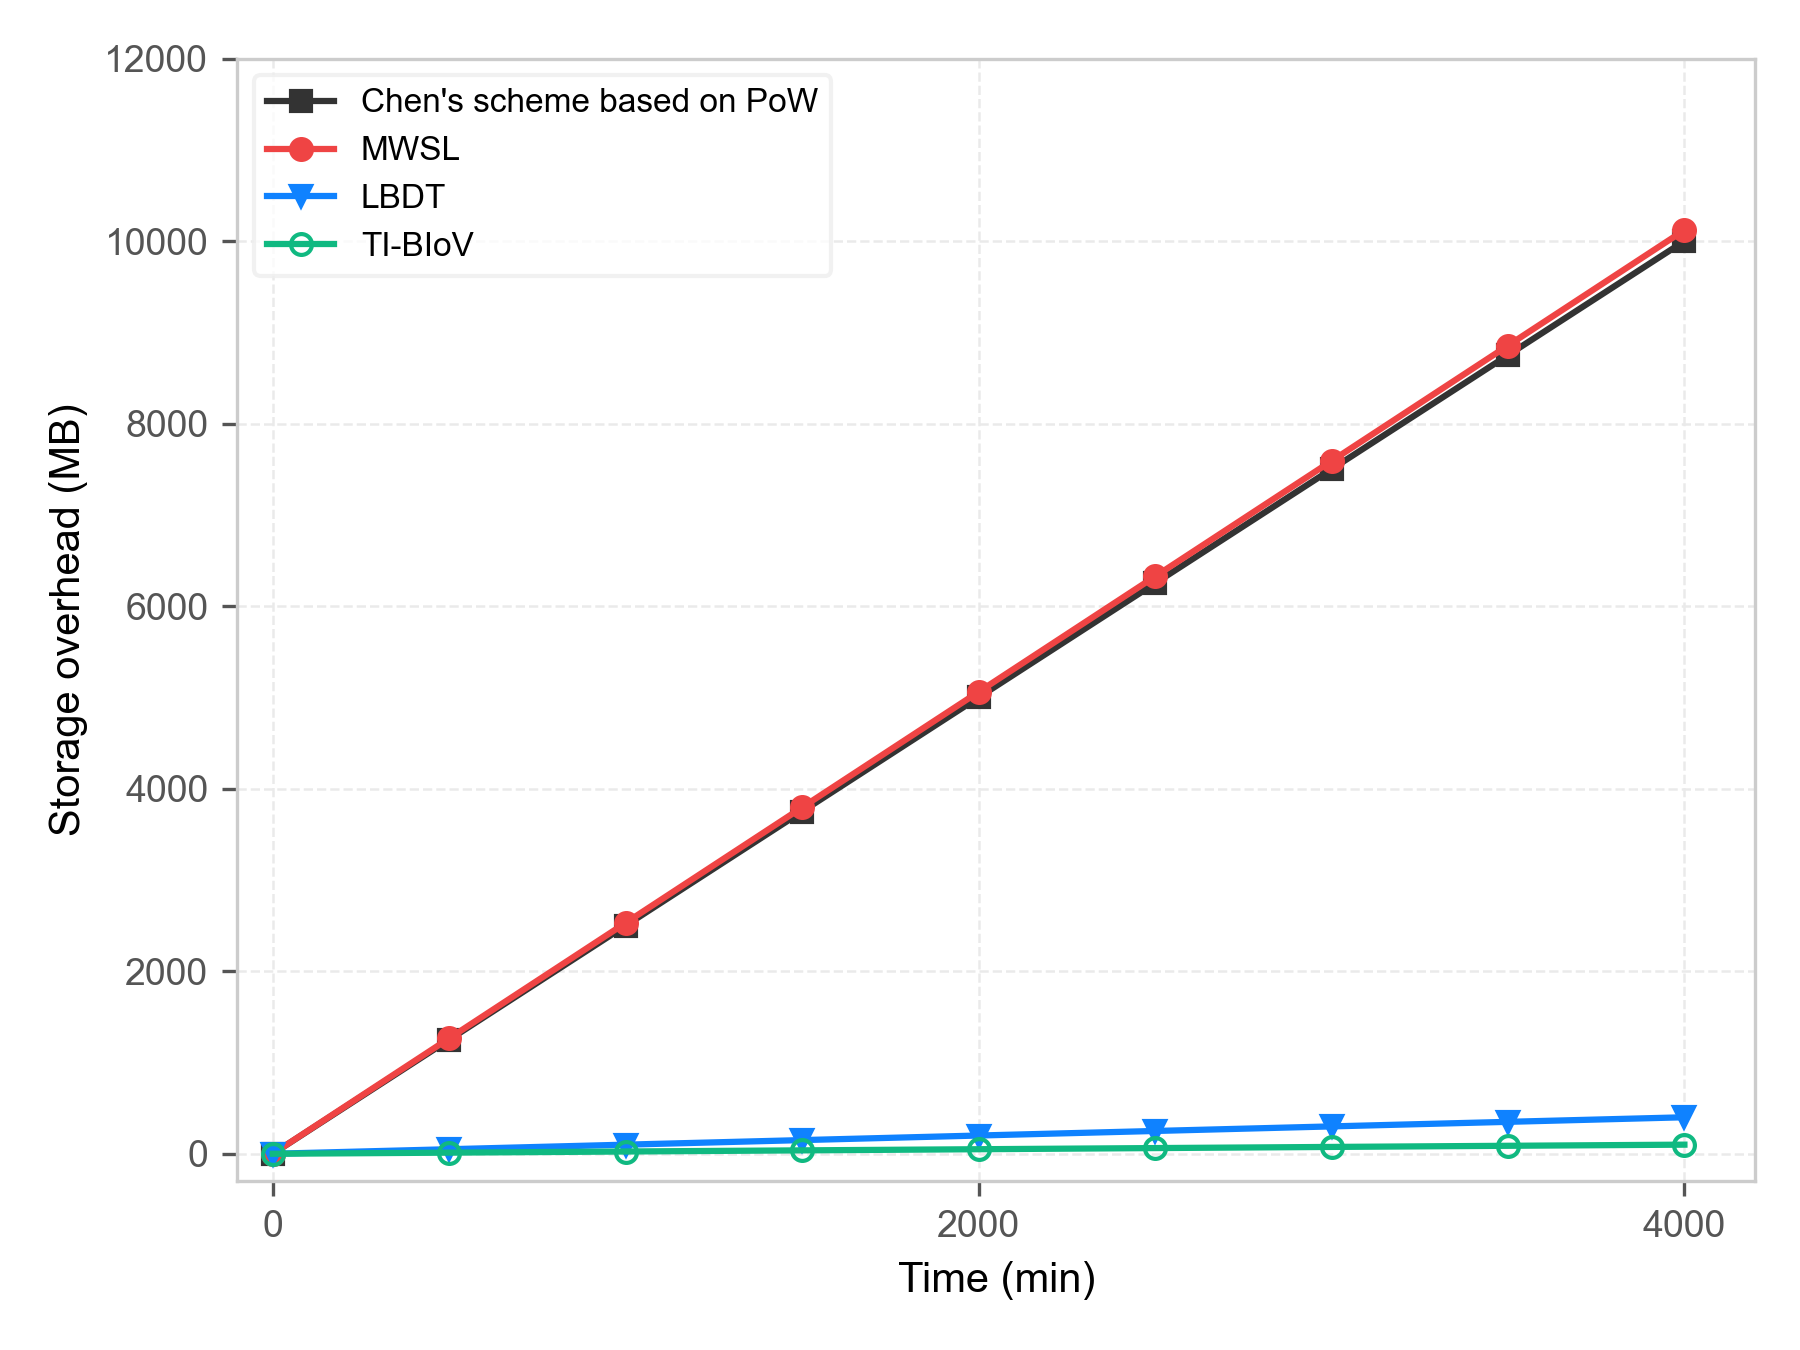
\includegraphics[width=4.8in]{chapters/5/fig_13_storage.png}
\caption{Ledger Storage Growth Over Time for Microblocks and Keyblocks.}
\label{fig:storage_growth}
\end{figure}

\section{Comparative Evaluation}\label{sec:results_comparison}
\noindent Table~\ref{table:comparison} presents a comprehensive comparative analysis of LBDT against existing IoV data trading and blockchain benchmarks.

\begin{table}[htbp]
\centering
\caption{Comparative Analysis of LBDT Against Baseline Vehicular Data Trading Schemes}
\label{table:comparison}
\renewcommand{\arraystretch}{1.4}
\resizebox{\textwidth}{!}{
\begin{tabular}{|l|c|c|c|c|c|}
\hline
\textbf{Data Trading Scheme} & \textbf{Avg Latency (s)} & \textbf{BFT Complexity} & \textbf{Reputation Model} & \textbf{ML Integration} & \textbf{Dynamic Sharding} \\ \hline
Monolithic PoW Blockchain \cite{nakamoto2008bitcoin} & $> 600.0$ & N/A (PoW) & None & No & No \\ \hline
SpeedyChain \cite{michelin2018speedychain} & $12.5$ & $O(N^2)$ & Static Scoring & No & No \\ \hline
Consortium IoV Scheme \cite{kang2019toward} & $8.4$ & $O(N^2)$ & Weighted Average & No & Static Zones \\ \hline
CHChain Crowdsourcing \cite{javaid2020scalable} & $5.1$ & $O(N \log N)$ & Static Threshold & No & No \\ \hline
\textbf{Proposed LBDT Scheme} & \textbf{2.4828} & \textbf{$5N-3$} & \textbf{Aged Gompertz} & \textbf{Logistic Reg (0.9991)} & \textbf{Dynamic ($U_z$)} \\ \hline
\end{tabular}
}
\end{table}